% --------------------------------------------------------------------------- %
% Poster for the ECCS 2011 Conference about Elementary Dynamic Networks.      %
% --------------------------------------------------------------------------- %
% Created with Brian Amberg's LaTeX Poster Template. Please refer for the     %
% attached README.md file for the details how to compile with `pdflatex`.     %
% --------------------------------------------------------------------------- %
% $LastChangedDate:: 2011-09-11 10:57:12 +0200 (V, 11 szept. 2011)          $ %
% $LastChangedRevision:: 128                                                $ %
% $LastChangedBy:: rlegendi                                                 $ %
% $Id:: poster.tex 128 2011-09-11 08:57:12Z rlegendi                        $ %
% --------------------------------------------------------------------------- %
\documentclass[a0paper,portrait]{baposter}

\usepackage{relsize}		% For \smaller
\usepackage{url}			% For \url
\usepackage{epstopdf}	    % Included EPS files automatically converted to PDF to include with pdflatex
\usepackage{cite}
\usepackage{xcolor}
\usepackage{caption}
\usepackage{float}
\usepackage[caption = false]{subfig}
\usepackage[demo]{graphicx}

\newcommand{\tabref}[1]{Table~\ref{#1}}
\newcommand{\tabincell}[2]{\begin{tabular}{@{}#1@{}}#2\end{tabular}}
%%% Global Settings %%%%%%%%%%%%%%%%%%%%%%%%%%%%%%%%%%%%%%%%%%%%%%%%%%%%%%%%%%%

\graphicspath{{figures/}}	% Root directory of the pictures 
\tracingstats=2			% Enabled LaTeX logging with conditionals

%%% Color Definitions %%%%%%%%%%%%%%%%%%%%%%%%%%%%%%%%%%%%%%%%%%%%%%%%%%%%%%%%%

\definecolor{bordercol}{RGB}{40,40,40}
\definecolor{headercol1}{RGB}{186,215,230}
\definecolor{headercol2}{RGB}{80,80,80}
\definecolor{headerfontcol}{RGB}{0,0,0}
%\definecolor{boxcolor}{RGB}{186,215,230}
\definecolor{boxcolor}{RGB}{255,255,255}
%%%%%%%%%%%%%%%%%%%%%%%%%%%%%%%%%%%%%%%%%%%%%%%%%%%%%%%%%%%%%%%%%%%%%%%%%%%%%%%%
%%% Utility functions %%%%%%%%%%%%%%%%%%%%%%%%%%%%%%%%%%%%%%%%%%%%%%%%%%%%%%%%%%

%%% Save space in lists. Use this after the opening of the list %%%%%%%%%%%%%%%%
\newcommand{\compresslist}{
	\setlength{\itemsep}{1pt}
	\setlength{\parskip}{0pt}
	\setlength{\parsep}{0pt}
}

%%%%%%%%%%%%%%%%%%%%%%%%%%%%%%%%%%%%%%%%%%%%%%%%%%%%%%%%%%%%%%%%%%%%%%%%%%%%%%%
%%% Document Start %%%%%%%%%%%%%%%%%%%%%%%%%%%%%%%%%%%%%%%%%%%%%%%%%%%%%%%%%%%%
%%%%%%%%%%%%%%%%%%%%%%%%%%%%%%%%%%%%%%%%%%%%%%%%%%%%%%%%%%%%%%%%%%%%%%%%%%%%%%%

\begin{document}
\typeout{Poster rendering started}

%%% Setting Background Image %%%%%%%%%%%%%%%%%%%%%%%%%%%%%%%%%%%%%%%%%%%%%%%%%%
\background{
	\begin{tikzpicture}[remember picture,overlay]%
	\draw (current page.north west)+(-2em,2em) node[anchor=north west]
	{};
        %{\includegraphics[height=1.1\textheight]{background}};
	\end{tikzpicture}
}

%%% General Poster Settings %%%%%%%%%%%%%%%%%%%%%%%%%%%%%%%%%%%%%%%%%%%%%%%%%%%
%%%%%% Eye Catcher, Title, Authors and University Images %%%%%%%%%%%%%%%%%%%%%%
\begin{poster}{
	grid=false,
	%eyecatcher=false, 
	borderColor=bordercol,
	headerColorOne=headercol1,
	headerColorTwo=headercol2,
	headerFontColor=headerfontcol,
	boxColorOne=boxcolor,
	headershape=roundedright,
	headerfont=\Large\sf\bf,
	textborder=rectangle,
	background=user,
        %background=plain,
	headerborder=open,
        boxshade=plain,
        bgColorOne=white
}

%%% Eye Cacther %%%%%%%%%%%%%%%%%%%%%%%%%%%%%%%%%%%%%%%%%%%%%%%%%%%%%%%%%%%%%%%
%{
%	Eye Catcher, empty if option eyecatcher=false - unused
%}
%%% Title %%%%%%%%%%%%%%%%%%%%%%%%%%%%%%%%%%%%%%%%%%%%%%%%%%%%%%%%%%%%%%%%%%%%%
{\sf\bf Automatic Soft CGRA Customization for High-Productivity 
Nested Loop Acceleration on FPGAs 
}
%%% Authors %%%%%%%%%%%%%%%%%%%%%%%%%%%%%%%%%%%%%%%%%%%%%%%%%%%%%%%%%%%%%%%%%%%
{
	\vspace{1em} Cheng Liu, Hayden Kwok-Hay So\\
    Department of Electrical and Electronic Engineering \\
    The University of Hong Kong
	%{liucheng@eee.hku.hk, hso@eee.hku.hk}
}
%%% Logo %%%%%%%%%%%%%%%%%%%%%%%%%%%%%%%%%%%%%%%%%%%%%%%%%%%%%%%%%%%%%%%%%%%%%%
{
% The logos are compressed a bit into a simple box to make them smaller on the result
% (Wasn't able to find any bigger of them.)
\setlength\fboxsep{0pt}
\setlength\fboxrule{0pt}
  \fbox{
    \begin{minipage}{12em}
    \includegraphics[width=12em,height=12em]{hkulogo}
    \end{minipage}
  }
}

\headerbox{Introduction}{name=motivation,column=0,row=0}{
Compiling high level compute kernels 
to FPGAs via an abstract overlay architecture 
is an effective way to 
improve designers' productivity. 
However, achieving the desired performance and 
overhead constraints requires exploration in a 
complex design space involving multiple 
architectural parameters and counteracts 
the benefit of utilizing an overlay 
as a productivity enhancer.

To address the above problem, a soft CGRA (SCGRA) with 
regular tiling structure is used an FPGA overlay. Because of the regularity  
of the SCGRA overlay, design metrics such as power consumption, implementation 
frequency are highly predictable and the system customization problem can be 
reduced to a simpler sub design space exploration (DSE) centering SCGRA 
scheduling and a straightforward customization with all the potential 
configurations well estimated using analytical models. 
With the proposed customization framework, we can achieve both high 
design productivity and performance.
}

\headerbox{SCGRA based accelerator}{name=scgra, column=0, below=motivation}{
\vspace{-1em}
\begin{figure}[H]
    \centering
    \float{\includegraphics[width = 0.88\linewidth]{scgra-accelerator}}
    \caption{SCGRA based FPGA accelerator}
    \label{fig:scgra-acc}
\end{figure}

\vspace{-2em}
\begin{figure}[H]
    \centering
    \float{\includegraphics[width = 0.88\linewidth]{pe}}
    \caption{PE structure}
    \label{fig:pe}
\end{figure}
\vspace{-1em}
}


\headerbox{FPGA acceleration framework}{name=loopacc,column=1,row=0}{
QuickDough--a rapid FPGA acceleration design framework using 
soft CGRA overlay is presented in Figure \ref{fig:loopacc-framework}.
\vspace{-0.2em}
\begin{figure}[H]
    \centering
    \float{\includegraphics[width = 0.9\linewidth]{framework}}
    \caption{QuickDough: a rapid FPGA acceleration design framework}
    \label{fig:loopacc-framework}
\end{figure}
}

\headerbox{Customization framework}{name=customization,column=1,row=1,below=loopacc}{
The customization is a critical part of QuickDough.
By taking advantage of the regularity of the SCGRA overlay, 
the complex nested loop acceleration problem is greatly 
simplified and divided into two simpler steps as shown in 
Figure \ref{fig:customization-framework}.  

\vspace{-0.5em}
\begin{figure}[H]
    \centering
    \float{\includegraphics[width = 0.97\linewidth]{customization-framework}}
    \caption{Customization framework for nested loop acceleration}
    \label{fig:customization-framework}
\end{figure}

}

\headerbox{Experiment setup}{name=setup, row=2, above=bottom}{
We took four applications including Matrix multiplication (MM), FIR, Kmean(KM), 
and Sobel edge detector (SE) as our benchmark. The detailed configuration of the 
benchmark is listed in the following table.
\vspace{-0.5em}
\begin{table}[H]
    \centering
    \begin{tabular}{l|l}
        \hline
        Benchmark & Parameters  \\ \hline
        MM & Matrix Size(128) \\ \hline
        FIR & \tabincell{l}{\# of Input (1024) \\ \# of Taps+1 (64)} \\ \hline
        SE & \tabincell{l}{ \# of Vertical Pixels (128) \\ \# of Horizontal Pixels (8)} \\ \hline 
        KM & \tabincell{l}{\# of Nodes(1024) \\ \# of Centroids(4) \\ \# of Dimensions(2)} \\ \hline  
    \end{tabular}
\end{table}

}

\headerbox{Experiment results}{name=experiment1,column=2,row=0}{
The customization problem is simplified with the observations in 
Figure \ref{fig:design-influence} and Figure \ref{fig:power-consumption}.

\vspace{-1.5em}
\begin{figure}[H]
    \centering
    \begin{tabular}{cc}
        \subfloat[Unrolling factor]{\includegraphics[width = 0.4\linewidth]{unrolling-perf}} &
        \subfloat[SCGRA size]{\includegraphics[width = 0.4\linewidth]{scgrasize-perf}}
    \end{tabular}
    \vspace{-1em}
    \caption{Design parameters influence on loop perforemance}
    \label{fig:design-influence}
\end{figure}
\vspace{-1em}

\vspace{-2em}
\begin{figure}[H]
    \centering
    \begin{tabular}{cc}
        \subfloat[BRAM power]{\includegraphics[width = 0.4\linewidth]{BRAM-Power}} &
        \subfloat[Power excluding BRAM power]{\includegraphics[width = 0.4\linewidth]{Base-Power}}
    \end{tabular}
    \vspace{-1em}
    \caption{Predictable power consumption of the SCGRA overlay based FPGA accelerators}
    \label{fig:power-consumption}
\end{figure}
\vspace{-1.2em}

The benchmark is implemented using both the proposed
two-step customization (TS) and exhaustive search (ES) customization.
Figure \ref{fig:DSE-Time} shows the DSE time comparison and Figure \ref{fig:pareto-curve} 
presents the Pareto-Optimal curve comparison. Figure \ref{fig:hls-cp} shows the 
benchmark performance of implementations using the proposed design framework and 
Vivado HLS.

\vspace{-0.5em}
\begin{figure}[H]
    \centering
    \float{\includegraphics[width = 0.7\linewidth]{DSE-Time}}
    \vspace{-0.5em}
    \caption{RA DSE time Vs. ES DSE time}
    \label{fig:DSE-Time}
\end{figure}
\vspace{-1em}

\vspace{-2em}
\begin{figure}[H]
    \centering
    \begin{tabular}{cc}
        \subfloat[MM]{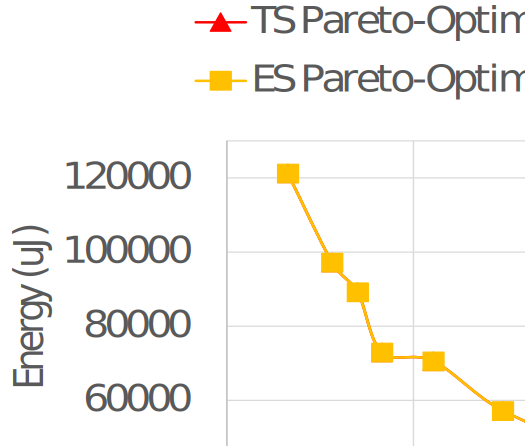
\includegraphics[width = 0.38\linewidth]{mm-energy-performance}} &
        \subfloat[FIR]{\includegraphics[width = 0.38\linewidth]{fir-energy-performance}} \\
        \subfloat[SE]{\includegraphics[width = 0.38\linewidth]{se-energy-performance}} &
        \subfloat[KM]{\includegraphics[width = 0.38\linewidth]{km-energy-performance}}
    \end{tabular}
    \vspace{-1em}
    \caption{Performance-energy Pareto-optimal curve comparison between RA DSE and ES DSE}
    \label{fig:pareto-curve}
\end{figure}
\vspace{-1em}

\vspace{-2em}
\begin{figure}[H]
    \centering
    \begin{tabular}{cc}
        \subfloat[MM]{\includegraphics[width = 0.38\linewidth]{mm-hls-cp}} &
        \subfloat[FIR]{\includegraphics[width = 0.38\linewidth]{fir-hls-cp}} \\
        \subfloat[SE]{\includegraphics[width = 0.38\linewidth]{se-hls-cp}} &
        \subfloat[KM]{\includegraphics[width = 0.38\linewidth]{km-hls-cp}}
    \end{tabular}
    \vspace{-1em}
    \caption{Performance comparison between the customized design and optimized HLS design}
    \label{fig:hls-cp}
\end{figure}
\vspace{-1em}


}
\headerbox{Conclusion}{name=conclusion, column=1, above=bottom}{
In this work, we have presented an automatic nested loop acceleration 
framework based on a homogeneous SCGRA overlay built on top of 
off-the-shelf FPGA devices. Given high level user constraints and design goals, 
the framework performs an intensive system customization specifically 
to a nested loop. According to the experiments, it can produces quite 
similar energy-performance Pareto-optimal curve to that obtained from 
an exhaustive search. The customized implementations exhibit competitive 
performance to the optimized HLS implementations.

}
\end{poster}
\end{document}
